\documentclass[onecolumn]{article}

\usepackage{times}
\usepackage{url}
\usepackage{graphicx}
\usepackage{abbrev}
\usepackage{color}
\usepackage{colortbl}

\usepackage{amssymb}
\usepackage{amsmath}
\usepackage{amsfonts}

\input{widen}
\input{macros}
\include{Acronym}


%%%%%%%%%%%%%%%%%%%%%%%%%%%%%%%%%%%%%%%%%%%%%%%%%%%%%%%%%%%%%%%%%%%%%%%%%%%
%%%%%%%%%%% Side By Side Macro   %%%%%%%%%%%%%%%%%%%%%%%%%%%%%%%%%%%%%%%%%%
%%%%%%%%%%%%%%%%%%%%%%%%%%%%%%%%%%%%%%%%%%%%%%%%%%%%%%%%%%%%%%%%%%%%%%%%%%%
\long\def\sidebyside#1#2{%
\hbox to\textwidth{\vtop{\hsize=.5\textwidth%
\advance\hsize by -.5\columnsep
\parindent=0pt
\centering

#1\vskip1sp}\hskip\columnsep\vtop{\hsize=.5\textwidth%
\advance\hsize by -.5\columnsep
\parindent=0pt
\centering
#2

}\hfill}}

\DeclareGraphicsExtensions{.png}

\title{\Large\bf
\vspace{-0.5in}
Adding Benchmarking Capabilities to PICML: User Guide
}

\author{
Arvind S. Krishna\\
\normalsize{arvindk@dre.vanderbilt.edu}\\
}
\date{}

\begin{document}
\maketitle

\section*{Introduction}

Platform Independent Component Modeling Language (or PICML, as it will
be called hereafter) is a graphical modeling language for the building
blocks of component applications, that is, applications that are built
on top of component middleware. It isn't intended to represent, or
conform to the specification of, any particular kind of middleware or
any particular vendor's product. Rather, it's an environment in which
to design and modify component applications in a way that's
technology-neutral, in a way that can be translated into the
middleware flavor of your choice. One such translator has already been
written, and is described in detail at the end of this document. More
are in the works.

PICML itself was designed using the Generic Modeling Environment
(GME), a powerful modeling tool developed at the Institute for
Software Integrated Systems (ISIS) at Vanderbilt University. Models in
PICML are also constructed using GME (I told you it was powerful),
since PICML itself can be registered with an installed copy of GME and
then selected from a list of modeling languages when starting a new
model project. Documentation, download and other information can be
found on the GME web page at:
\url{http://www.isis.vanderbilt.edu/Projects/gme/}

This document pertains to adding benchmarking capabilities to PICML
and discusses benchmark generation from higher level models. Using the
benchmarking code, metrics such as roundtrip latency and throughput
can be measured. This tool is designed as a helper tool and interacts
with other tools such as OCML (Options Configuration Modeling
Language) and PICML (deployment plan evaluation).  These tools are a
part of a larger tool-suite called Component Synthesis with Model
Integrated Computing CoSMIC. This document does not deal with the
motivation for the development of this capability, rather describes a
step-wise process of adding and composing simple benchmarks using
PICML models.

\section* {Installing PICML}

A Windows installer for PICML is available from the CoSMIC web page
listed above. Just look at the first item under the Downloads header
near the top of the page. The benchmarking capabilities are part of
PICML.

\section* {Prerequisites}
After installing PICML there are two steps that are
required before one can set up benchmarks.  These are common to
someone building models from scratch of existing PICML models. These
include:
\sqztiny
\begin{enumerate}\crunchlist
\item {\bf Component interactions:} Component instances and their ports.
\item {\bf Component interfaces:} The interfaces provided and required by
components.
\end{enumerate}

\noindent The BGML generated code uses several capabilities provided
by the ACE framework. ACE can be downloaded from
\url{http://deuce.doc.wustl.edu/Download.html}. Currently, all
generated code from BGML has been tested using the CIAO open-source
component middleware framework that runs atop ACE and TAO open-source
CORBA middleware. These can be downloaded from the url provided above.

\noindent The first step is provided via ComponentImplementation aspect in
PICML. In this view, the user can drag and drop components and draw
the component interactions. For more information please refer to the
user guide exclusively dealing with PICML. The second step is accomplished via
the ComponentTypes aspect in PICML. This aspect deals with specifying
the interfaces of the ports. Please refer to the Interfaced
Definitions manual present with the installation of PICML.

From this point, I assume that the models have both the component
interactions and component interfaces.  The assumption also includes
how to open an existing model, create a new model (PICML) in GME and
some GME terminology. For GME terminology, please refer to the GME
user manual.

\section*{BGML Model Elements}

This section describes the BGML modeling elements, both their syntax
and semantics. For the purpose of benchmarking, BGML provides the
following model elements:

\begin{description}\crunchlist
\item [{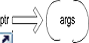
\includegraphics[width=1.5cm] {operationref.png}}]

Operation Reference points to a two way IDL operation. The actual
operation is defined in the ComponentTypes aspect of PICML. BGML
requires the signature of the operation to generate benchmarking code

\item [{
\includegraphics [width=1.5cm] {eventref.png}}]

Event Reference points to a CORBA event exchanged between one/many
components. Similar to operations, events are also defined in the
ComponentTypes aspect of PICML. The type of event is used by BGML to
generate benchmarking code

\item [{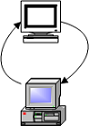
\includegraphics [width=1.5cm] {Latency.png}}]

Latency element is associated with an IDL operation/event. A latency
element can be associated with only one operation or an event. The
BGML model interpreter then uses this association to generate code the
measures the latency for each invocation of the operation/event. For
each latency element, the following three attributes to be associated:
\sqztiny
\begin{enumerate}\crunchlist
\item  {\bf filename:} Generates output a given file, later imported by a
graphing tool
\item {\bf warmup:} number of iterations to warmup before taking the actual
benchmark
\item {\bf iterations:} Number of iterations to compute latency measures
\end{enumerate}

\item [{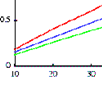
\includegraphics [width=1.5cm] {Throughput.png}}]

Throughput element similar to Latency is associated with an IDL
operation/event. Every throughput element can be associated with one
operation or event. Similar to the latency measures, the benchmarking
code generates the throughput measures. The same three attributes
associated with Latency can also be associated with throughput

\item [{
\includegraphics [width=1.5cm] {timer.png}}]

Time probe element can be used to generate timing information for both
IDL operations and CORBA events. The \url{start_time_probe ()} and
\url{stop_time_probe ()} functions generated from the BGML interpreters can
be used to take timestamps before and after method invocation. These
timestamps can then server as input to other timing analysis
tools. Every timeprobe element can be associated with many operations
and events.

\item [{
\includegraphics [width=1cm] {taskset.png}}]

Benchmarking experiments require some background load either CPU or
other requests during the benchmarking process. These make the results
more insightful. A TaskSet is a set of tasks that can be used to
create a certain number of background tasks during the benchmarking
experiment.

\item [{
\includegraphics [width=0.5cm] {task.png}}]

A task represents a background activity, in our case generation of
requests during the benchmarking process. These requests are remote
CORBA operations on the target server process. The number of
iterations are the same as the benchmarking operation. Each task set
can be associated with n (1..n) number of background tasks.

\end{description}

\section*{Getting Started with BGML}

Open PICML model and right click on the RootFolder. This opens up a
dialog box. In this box choose Insert Folder. This should open up a
menu with different folders roughly corresponding to each aspect in
PICML. Choose the ComponentAnalyses aspect. This step is illustrated in
Figure~\ref{step1}.

\begin{figure}[ht]
\sidebyside {
  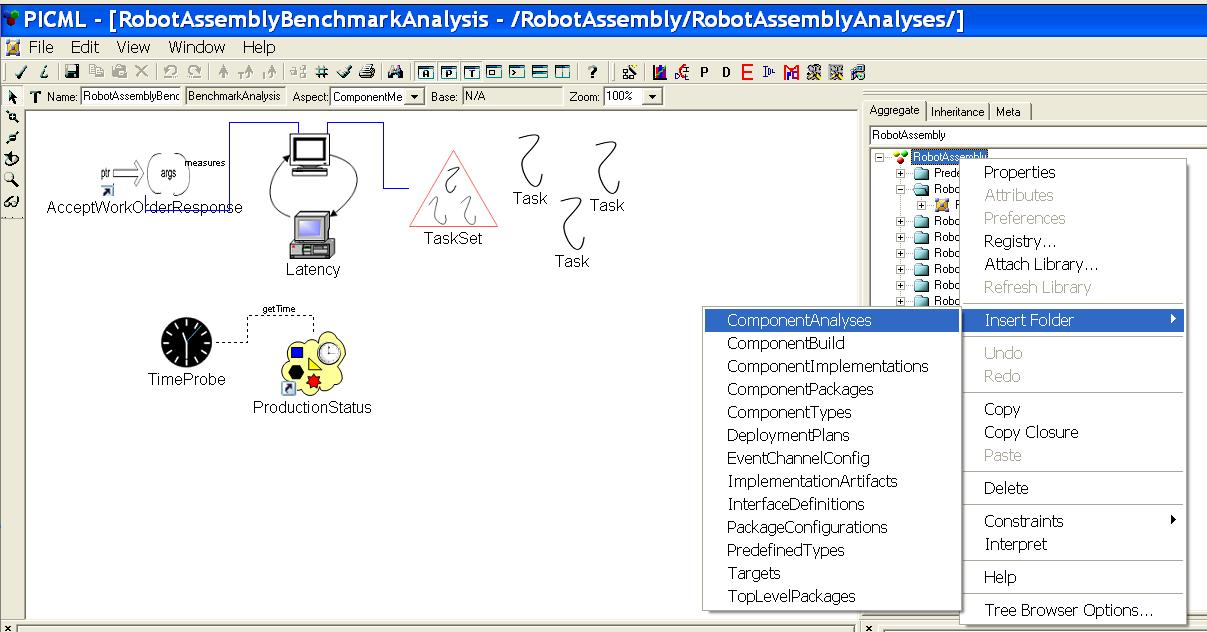
\includegraphics[width=7cm]{InsertFolder.png}
   \bfcaption{Step 1}
   \label{step1}
}
{
 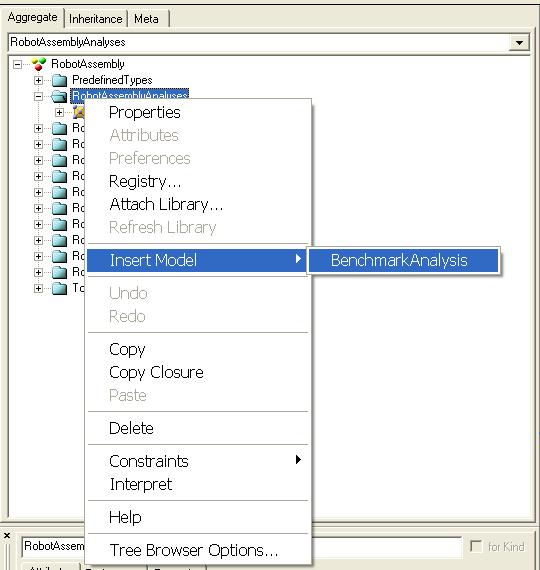
\includegraphics[width=5cm]{Insert-Benchmark.png}
  \bfcaption{Step 2}
  \label{step2}
}
\end{figure}

Step 1 should create a NewComponentAnalyses folder. Right click
on this to insert a BenchmarkAnalysis Model. Currently there is only
one model or one type of analysis. In future, there might be different
analysis such as one that is specific for MatLab. In that case, there
will be two types, one for Benchmark another for Matlab. This step is
shown in Figure~\ref{step2}. Steps 1 \& 2 enable creation of a BGML
paradigm for modeling benchmarks. After these steps you should see the
screen as shown in Figure~\ref{step3}.

\begin{figure}[htpb]
\center{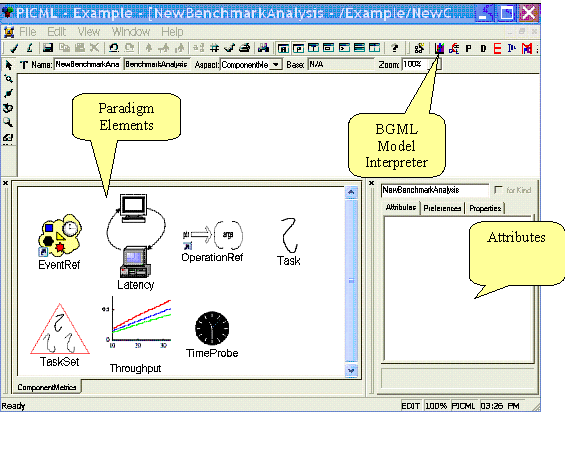
\includegraphics[width=7cm]{New_Paradigm.png}}
\bfcaption{BGML Paradigm Window}
\label{step3}
\end{figure}

If not, please go over Steps 1 and 2 to see what went wrong.  To set
up a simple benchmark, BGML requires the signature of the IDL
operation or an Event that has to be benchmarked. Either of these
are to be modeled in the Interface Definitions aspect present in PICML.

\section* {Creating Benchmarking Experiments: A Walk Through}
In this section, I describe how to create a benchmarking experiment
with PICML. The example discussed is a part of the RobotAssembly
example shipped with the PICML installation present in:
\url{\$COSMIC_ROOT/examples/RobotAssembly.xme}. Similar steps can be
followed to create other benchmarks.

In this scenario, a pallet (controlled by a {\tt Palette\-Manager}
component) containing digital watches moves to a robot station
(controlled by the {\tt Robot\-Manager} component) where its time is
set using the current time provided by a periodic clock (controlled by
a {\tt Watch\-Manager}).  The management for the watch setting
facility located at a remote site can send production work orders and
receive response to orders, ongoing work status, inventory, and other
messages. These instructions are sent to the {\tt Watch\-Manager}
component using {\tt Management\-Work\-Instructions} ({\tt MWI})
component. The {\tt Watch\-Manager} component interacts with a human
operator who using the {\tt Human\-Machine\-Interface} ({\tt HMI})
component accepts/rejects the watch.  When the watch is accepted, the
{\tt Watch\-Manager} component uses the {\tt Robot\-Manager} component
to set the time.  When a watch is rejected, however, the {\tt
Robot\-Manager} component removes the watch from the assembly line.
Figure~\ref{fig:robotassembly} illustrates this assembly of
components.

\begin{figure}[htpb]
\begin{center}
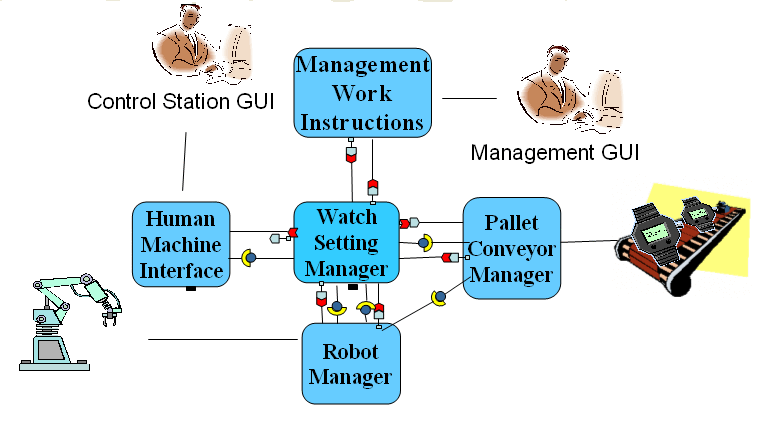
\includegraphics[width=5cm]{RobotAssembly.png}
\bfcaption{RobotAssembly Scenario}
\label{fig:robotassembly}
\end{center}
\end{figure}

Figure~\ref{interaction} depicts the interaction between the
components in the RobotAssembly scenario using PICML. The details on
how to model the scenario in PICML is external to this document. More
details should be available from the PICML documentation guide. As
shown in the figure, \url{HumanMachineInterface} and
\url{WatchSettingManager} component interact via a
facet(\url{DisplayResponse}) receptacle (\url{HumanResponse})
communication.

\begin{figure}[ht]
\sidebyside {
  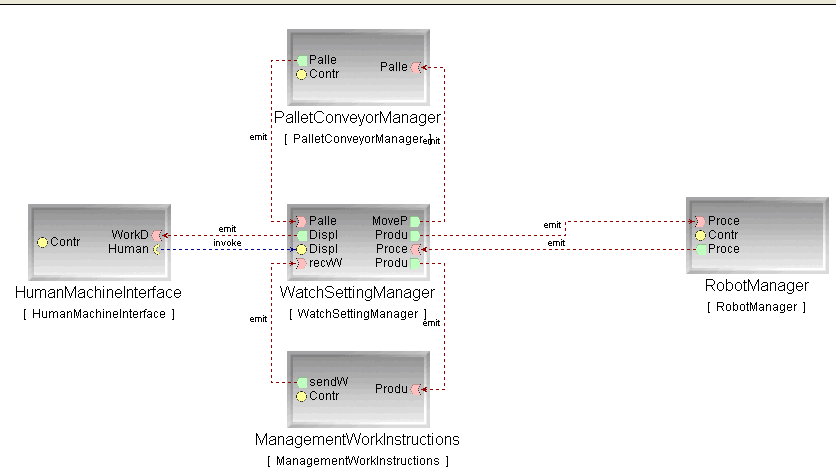
\includegraphics[width=7cm]{RobotAssembly-Intr.png}
   \bfcaption{RobotAssembly Interaction Scenario}
    \label{interaction}
}
{
  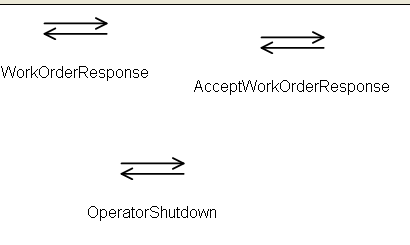
\includegraphics[width=6cm]{RobotAssembly-Operations.png}
   \bfcaption{Operations part Facet/Receptacle Interaction}
    \label{operations}
}
\end{figure}
Figure~\ref{operations} shows three operations part of the interface
exchanged between \url{HumanMachine\-Interface} and
\url{WatchSettingManager} components. The relevant IDL is shown below:
{
\small
\ls{0.8}
\begin{verbatim}
interface  WorkOrderResponses {
 void AcceptWorkOrderResponse(in WorkOrder Order, in StatusType Status);
 void SetTimeResponse(in WorkOrder Order, in StatusType Status);
 void AcceptFinalProductResponse(in WorkOrder Order, in StatusType Status);
};
\end{verbatim}
}
\normalsize

{\bf NOTE:} As stated earlier, modeling components, interfaces and their
operations and part of the PICML documentation and are not explicitly
discussed in this document. Please consult the Interface Definitions
documentation and PICML documentation for a detailed description.

At this point, we are ready to create an experiment that measures the
roundtrip latency for the \url{AcceptWorkOrderResponse} method. The
following is a step wise description:

\smallskip
\noindent {\bf Step 1:} Copy the \url{AcceptWorkOrderResponse} operation
present in the InterfaceDefinitions aspects of the RobotAssembly model
and paste it in the RobotAssembly benchmark paradigm. Creation of the
benchmark paradigm can be done from the first two steps explained in
Getting Started with BGML section. This step is shown in
Figure~\ref{bgml-copy}.

\begin{figure}[ht]
\sidebyside {
 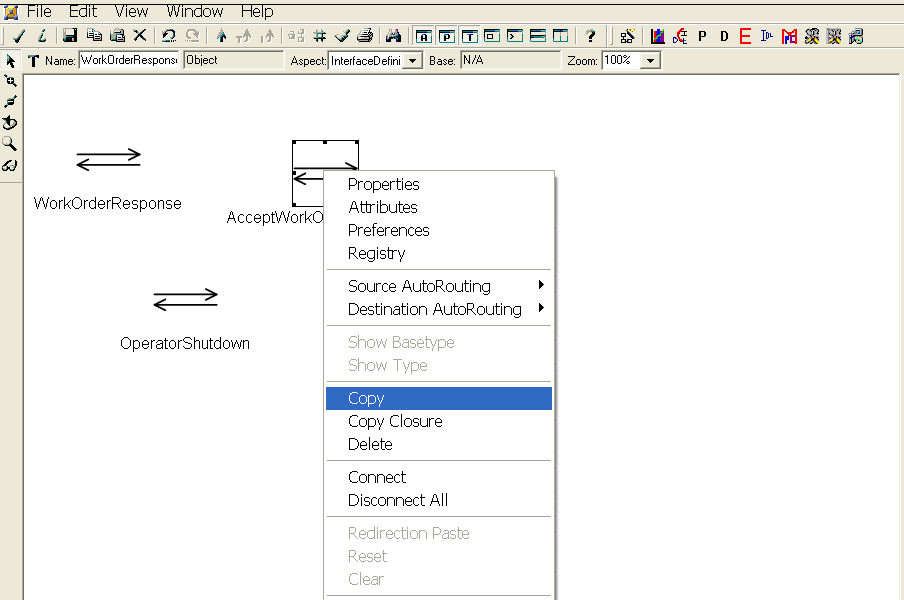
\includegraphics[width=7cm]{RobotAssembly-OperationCopy.png}
 \bfcaption{Copying Operation Signature onto BGML}
 \label{bgml-copy}
}
{
 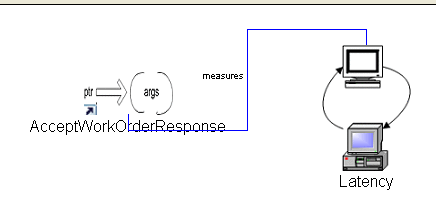
\includegraphics[width=5cm]{BGML-Latency.png}
 \caption{Associating Round-trip Latency with Operation}
 \label{bgml-latency}
}
\end{figure}

\smallskip
\noindent {\bf Step 2:} Once the operation signature has been copied,
associate either Latency or Throughput metric with this operation. In
our case, we drag the latency icon from the palette and drop onto the
pane. Then using the {\em Connect Mode} provided by GME, associate the
operation with the Latency Metric. This is done by selecting the
source, (operation reference) and the sink (latency element) one at a
time. Figure~\ref{bgml-latency} shows the resulting step.

\begin{figure}[ht]
\sidebyside {
 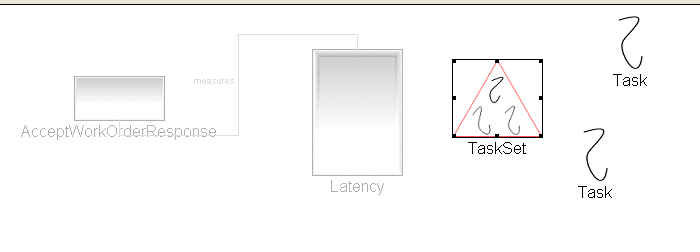
\includegraphics[width=7cm]{BGML-Task-Assoc.png}
 \bfcaption{Associating Tasks with TaskSet}
 \label{task-association}
}
{
 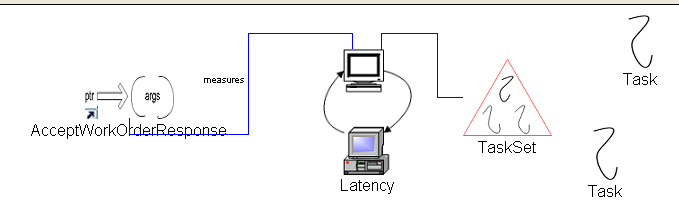
\includegraphics[width=7cm]{BGML-Latency-Complete.png}
 \bfcaption{Associating Task Set with Latency Metric}
 \label{task-complete}
}
\end{figure}

\smallskip
\noindent {\bf Step 3:} Select the Latency Metric to configure the
attributes, {\em i.e.}, the number of warmup iterations and number of
actual iterations. This can be configured using the attributes.

\smallskip
\noindent {\bf Step 4:} Associate a predetermined number of background tasks
with the experiment. To do this first drag a task set element from the
palette. Next, drag and drop the required number of background tasks
using the task element in the palette. Associate each of these tasks
with the task set. For doing this use the {\em Set Mode} provided in
GME and select the individual tasks to be part of the task set. This
is shown in Figure~\ref{task-association}. Next using the {\em Connect Mode}
connect the latency metric with the task set.

\paragraph* {\bf Checking Constraints.}
Once this is done. Please check for constraint violations. This can be
done by choosing. File$\rightarrow$Check$\rightarrow$Check All
constraints from the File menu in GME. There should not be any
constraint violations. The final experiment visually should look like
what is shown in Figure~\ref{task-complete}. If there are any, please
see if they pertain to the BGML paradigm and revisit steps 1-4 to
ensure you have followed all the steps. If there are still violations,
please export the GME model via File$\rightarrow$Export XML and send the
resulting file to arvindk@dre.vanderbilt.edu If there are no
violations you are ready to interpret the file and look at the
generated code. This step is discussed in the next section. Similar
steps can be followed for events.

\paragraph* {\bf Associating Timer probes:}
To associate a timer probe connection with either an operation or an
event, follow Step 1 described earlier. Next drag and drop the Timer
element and create a connection between the operation/event with the
timer probe. This should be done using the {\em Connect Mode} as
described earlier.  A single timer atom can be connected to multiple
operations or events. After this association, please follow
instructions on how to check constraints via {\em Checking
Constraints} section explained earlier.

\section* {Generated Code: A Walk Through}
Having built the models, the next step is to invoke the interpreter to
generate the required benchmarking code. There are several
interpreters in GME, one can look at all the interpreters by clicking
the {\bf i} icon present in the GME toolbar. Alternatively, one can
directly invoke the BGML interpreter by choosing the BGML interpreter
icon as shown in Figure~\ref{step3}. All the generated code from BGML
uses several classes provided by the ACE framework including,
Barriers, Threads, and priority mechanisms. The use of ACE ensures
that the generated code from BGML can be run across different
platforms and compilers. ACE is freely available and can be downloaded
from \url{http://deuce.doc.wustl.edu/Download.html}. This also means
that currently BGML generates C++ code. We do plan to generate java
benchmarking code as well. If you are interested or need this
functionality please email me at arvindk@dre.vanderbilt.edu. Next
a description of the generated code is provided.

\subsection* {Benchmark Header \& Source Files}
The interpreter generates header and source files that have
``Benchmark'' followed by ``Operation Name'' as their names. For the
examples the files generated include
Benchmark\_AcceptWorkOrder\-Response.\{h/cpp\}. Below we show the structure
of the generated code. This is done as it is important in our case to
understand what the actual benchmarking code looks like.

\subsection* {Header File}
{
\footnotesize
\begin{verbatim}
1:#ifndef BENCHMARK_ACCEPTWORKORDERRESPONSE_H
2: #define BENCHMARK_ACCEPTWORKORDERRESPONSE_H

3: #include "BGML_Task_Base.h"
4: #include "HumanMachineInterface_exec.h"
5: #include "Benchmark_AcceptWorkOrderResponse_export.h"

6: template <typename T>
7: BENCHMARK_ACCEPTWORKORDERRESPONSE_Export class
8: Benchmark_AcceptWorkOrderResponse : public BGML_Task_Base
9: {
10:  public:
11:    Benchmark_AcceptWorkOrderResponse (T* remote_ref,
12:                                       const RobotAssembly::WorkOrder& arg0,
13:                                       RobotAssembly::StatusType arg1);

14:    ~Benchmark_AcceptWorkOrderResponse ();
15:    int svc (void);

16:  protected:
17:    T* remote_ref_;
18:    const RobotAssembly::WorkOrder & arg0_;
19:    RobotAssembly::StatusType arg1_;
20: };

#include "Benchmark_AcceptWorkOrderResponse.cpp"
#endif // BENCHMARK_ACCEPTWORKORDERRESPONSE_H
\end{verbatim}
}
\normalsize

Lines 3--5 illustrate the include files required. All the benchmarking
classes inherit from \url{BGML_Task_Base} class. This class inherits
from \url{ACE_Task_Base} which enables the Benchmark class to be
associated with a thread. The \url{Human_MachineInterface_exec.h}
declares the signature for operation to be benchmarked. Lines 6--8
illustrate the class definition. The class itself is generic and requires
a type T. This type corresponds to the type of the remote interface.
Lines 10 -- 13 describes the constructor. The constructor take in three
arguments, each corresponding to the arguments required by the remote
operations. In our case the operation signature was:
{\tt AcceptWorkOrderResponse(in WorkOrder Order, in StatusType Status);}
The signature of the operation corresponds to the CORBA mapping of IDL
operation. The T* remote\_ref is a pointer to the remote interface on which
the operation will be invoked. The {\tt svc ()} method shown in Line 15
is the actual function in which the benchmarking is done. This function
also serves as the entry point for a thread associated with the benchmarking
class.

\subsection* {Benchmarking source file}

{
\footnotesize
\begin{verbatim}

#ifndef BENCHMARK_ACCEPTWORKORDERRESPONSE_C
#define BENCHMARK_ACCEPTWORKORDERRESPONSE_C

#include "Benchmark_AcceptWorkOrderResponse.h"
#include "ace/High_Res_Timer.h"
#include "ace/Stats.h"
#include "ace/Sample_History.h"
#include "AcceptWorkOrderResponse_Workload.h"

template <typename T>
int
Benchmark_AcceptWorkOrderResponse<T>::svc (void)
{

  for (int warm_up = 0; warm_up < 100; warm_up++)
    (void) this->remote_ref_->
      AcceptWorkOrderResponse (arg0_,arg1_ ACE_ENV_ARG_PARAMETER);

  ACE_Barrier barrier (3);

  // Generate the Background workload
  AcceptWorkOrderResponse_Workload<T> task0 (remote_ref_, arg0_, arg1_, barrier);
  AcceptWorkOrderResponse_Workload<T> task1 (remote_ref_, arg0_, arg1_, barrier);
  AcceptWorkOrderResponse_Workload<T> task2 (remote_ref_, arg0_, arg1_, barrier);

  // Activate the Background tasks
  if (task0.activate (THR_NEW_LWP | THR_JOINABLE, 1, 1) == -1)
    ACE_ERROR ((LM_ERROR, "Error activating workload task0 \n"));
  if (task1.activate (THR_NEW_LWP | THR_JOINABLE, 1, 1) == -1)
    ACE_ERROR ((LM_ERROR, "Error activating workload task1 \n"));
  if (task2.activate (THR_NEW_LWP | THR_JOINABLE, 1, 1) == -1)
    ACE_ERROR ((LM_ERROR, "Error activating workload task2 \n"));

  ACE_Sample_History history (5000);
  ACE_hrtime_t test_start = ACE_OS::gethrtime ();

  ACE_UINT32 gsf = ACE_High_Res_Timer::global_scale_factor ();
  for (int i = 0; i < 5000; i++)
  {
    ACE_hrtime_t start = ACE_OS::gethrtime ();
    (void)this->remote_ref_->
      AcceptWorkOrderResponse (arg0_,arg1_ ACE_ENV_ARG_PARAMETER);
    ACE_CHECK;
    ACE_hrtime_t now = ACE_OS::gethrtime ();

    history.sample (now - start);
  }

  ACE_hrtime_t test_end = ACE_OS::gethrtime ();
  ACE_DEBUG ((LM_DEBUG, "test finished"));
  ACE_DEBUG ((LM_DEBUG, "High resolution timer calibration...."));
  ACE_DEBUG ((LM_DEBUG, "done"));
  ACE_Basic_Stats stats;
  history.collect_basic_stats (stats);
  stats.dump_results ("Total", gsf);
  ACE_Throughput_Stats::dump_throughput ("Total",
                                         gsf,
                                         test_end - test_start,
                                         stats.samples_count ());
  return 1;
}
#endif // BENCHMARK_ACCEPTWORKORDERRESPONSE_H

\end{verbatim}
}
\normalsize
As illustrated in the code snippet, the \url{svc ()} method first
warms up the system by invoking the required number of warmup
iterations. Based on the number of background tasks modeled, in our
case 3, the interpreter generates three
\url{AcceptWorkOrderResponse_Workload} background tasks each of which send
requests concurrently when the actual benchmarking operation is
done. The next step activates each of these tasks. Once the background
tasks are activated, the actual benchmarking code to measure the round
trip latency is generated. Finally, after computing the results, the
statistics are displayed.

\subsection* {Build file}
The model interpreter also generates a build file to compile the
generated benchmark code and create a shared library that can be
linked to the actual application that requires this functionality. The
build files use MPC (Make Project Creator) which generates the
required Makefiles or Visual C++ build files. MPC is available for
download from OCI via \url{http://www.ociweb.com/product/mpc/}. We
provide the build file for sake of completeness. The next section
describes how one can build and run the benchmarks.

{
\footnotesize
\begin{verbatim}
project (Benchmark_AcceptWorkOrderResponse) : acelib , ciao_client {
  includes += $(BGML_HOME)
  libs     += BGML_Base
  libpaths += $(BGML_HOME)
  Source_Files {
    AcceptWorkOrderResponse_Workload.cpp
    Benchmark_AcceptWorkOrderResponse.cpp
  }
}
\end{verbatim}
}
\normalsize

\subsection* {Running Benchmarks Generated from BGML}
In this section I describe how the benchmarking files generated from
BGML can be run. These examples were tested on the DAnce open-source
component middleware. To compile the benchmarks first one needs to
compile the BGML\_Base directory shipped with PICML installation. Move
the sources to a directory for example:
\\build/arvindk/software/BGML\_Base.  Next set up an environment
variable \$BGML\_HOME that points to this directory. Next run the mwc.pl
(MakeProjectCreator) file shipped with MPC to generate the build file.
After which compile the directory using the appropriate make command. Below
we show the compilation snippet using gmake on Linux platform.
{
\footnotesize
\begin{verbatim}
bash-2.05$ /build/arvindk/ACE_wrappers/bin/mwc.pl
Generating gnuace output using default input
Start Time: Fri Nov 19 11:42:53 2004
  End Time: Fri Nov 19 11:42:53 2004

bash-2.05b$ make
make[1]: Entering directory `/build/arvindk/CoSMIC/PIM/PICML/interpreters/BGML_Base'

GNUmakefile:
/build/arvindk/CoSMIC/PIM/PICML/interpreters/BGML_Base/GNUmakefile.BGML_Base
MAKEFLAGS=w

g++ -W -Wall -Wpointer-arith -O3 -g -pipe -D_REENTRANT
-DACE_HAS_AIO_CALLS -D_GNU_SOURCE -I/build/arvindk/ACE_wrappers
-DACE_HAS_EXCEPTIONS -D__ACE_INLINE__ -I/build/arvindk/ACE_wrappers
-DBGML_BASE_BUILD_DLL -c -fPIC -o .shobj/BGML_Task_Base.o
BGML_Task_Base.cpp

g++ -D_REENTRANT -DACE_HAS_AIO_CALLS -D_GNU_SOURCE
-I/build/arvindk/ACE_wrappers -DACE_HAS_EXCEPTIONS -D__ACE_INLINE__
-I/build/arvindk/ACE_wrappers -DBGML_BASE_BUILD_DLL -shared -Wl,-h
-Wl,libBGML_Base.so.5.4.2 -o libBGML_Base.so.5.4.2
.shobj/BGML_Task_Base.o -Wl,-E -L/build/arvindk/ACE_wrappers/ace -L./
-L/build/arvindk/ACE_wrappers/lib -lACE -ldl -lpthread -lrt rm -f
libBGML_Base.so ln -s libBGML_Base.so.5.4.2 libBGML_Base.so chmod a+rx
libBGML_Base.so.5.4.2 Installing libBGML_Base.so ->
/build/arvindk/ACE_wrappers/lib Installing libBGML_Base.so.5.4.2 ->
/build/arvindk/ACE_wrappers/lib make[1]: Leaving directory
`/build/arvindk/CoSMIC/PIM/PICML/interpreters/BGML_Base'
\end{verbatim}
}

Next compile the benchmarking files. Copy the generated files to the
appropriate directory. In particular to the one where the
``HumaManchineInterface'' component is located. Follow similar steps
as describe earlier. Compilation generates
libBenchmark\_AcceptWorkOrderResponse.so library on a linux platform.

The final step is to invoke the benchmarking code from within the
component implementation to begin the benchmark. In particular, the
following lines of code should be added to the implementation:

{
\footnotesize

\begin{verbatim}
RobotAssembly::WorkOrderResponses_var rev = this->context_->
        get_connection_HumanResponse (ACE_ENV_SINGLE_ARG_PARAMETER);
      ACE_CHECK;

if (CORBA::is_nil (rev.in ()))
  ACE_THROW (CORBA::BAD_INV_ORDER ());

Benchmark_AcceptWorkOrderResponse<RobotAssembly::WorkOrderResponses>
benchmark (rev.in (), myOrder, myStatus);

if (benchmark.activate (THR_NEW_LWP|THR_JOINABLE, 1, 1) == -1)
  ACE_ERROR ((LM_ERROR, "Error activating workload task0 \n"));

\end{verbatim}
}

The first two lines shows how the remote reference to the interface
can be obtained via the provided facet. The next two lines show the
creation of a benchmarking task and passing in the required parameters
(myOrder and myStatus) which are defined earlier. Final step involves
activation of task which also starts the benchmarking experiment.
After adding this code, the user must link the application with
libBenchmark\_AcceptWorkOrderResponse.so library.

If there are any errors in the generated code, {\em i.e.}, runtime or
compilation errors please report them to arvindk@dre.vanderbilt.edu

\section* {Planned Feature Additions}
The following are some planned future additions:
\begin{enumerate}

\item Generate Java benchmarking code. This will be tailored towards
OpenCCM implementation.

\item Currently, all tasks are continuous {\em i.e.}, invoke operations at
the fastest possible rate. The future enhancement is to generate tasks
that invoke operations at a given rate or priority.

\item Integrate this tool with other CPU workload generators such as
Hourglass and CPU Broker. Please see the following URL for more
information: \url{http://www.cs.utah.edu/~regehr/hourglass/}.
\end{enumerate}

\section* {Summary}
This document dealt with modeling and generation of benchmarking
experiments using BGML. This tool automates the manual task of
generating benchmarks from models with very less overhead. The
generated code and the build files can be used to compile the files on
multiple platforms with no user modifications. We have used the tool
to quickly evaluate the performance of systems for a given configuration.
The configuration information generated from the OCML tool (part of the
CoSMIC tool chain). Similarly the tool can also be used to evaluate the
deployment plan, {\em i.e.}, how components map on to target nodes. Any
feedback, suggestion or criticism please direct to
Arvind S. Krishna arvindk@dre.vanderbilt.edu.

\end{document}
